\documentclass[12pt]{article}
%\usepackage{fancyvbr, pstcol}
%\setlength{\parskip}{1ex plus 0.5ex minus 0.2ex}
\setlength{\parskip}{1em}
\parindent0mm
\textwidth150mm
\textheight200mm
\oddsidemargin+5mm
%\usepackage[dvips]{graphicx}
\usepackage{color}
\usepackage[pdftex]{graphicx}
\definecolor{Light}{gray}{.80}
\setlength{\fboxrule}{1pt}
\setlength{\fboxsep}{2pt}

\begin{document}

\begin{titlepage}
\verb+      +
\vspace{3cm}
\begin{flushright}
{\huge\bf\verb+stkSolver+ User Guide}
\rule{150mm}{6pt}\\
\begin{large} v1.2, \today\\
\vspace{7cm}
{\bf by Carlos Rosales Fern\'andez}\\
Heterogeneous Coupled Systems\\
Institute of High Performance Computing\\
A*STAR, Singapore
\end{large}
\end{flushright}
\end{titlepage}
\pagebreak

\section*{Preface}\noindent \verb+stkSolver+ is a boundary element method solver for Stokes' equation in microfluidics problems. Version 1.2 supports only a single material and Dirichlet boundary conditions --given velocities. The discretization is done using isoparametric triangles, and both linear and quadratic elements are available. An indirect version of BEM is used in order to obtain equations which are numerically stable. The user can choose between an iterative GMRES solver with Jacobi preconditioner, a simple Gauss elimination solver, a Gauss-Jordan solver with full pivoting, or a LU decomposition solver. This manual describes mainly the correct structure of the input files. For any questions or comments contact the author at:\par\vspace{2em}

	Carlos Rosales Fern\'andez\hspace{1cm}\verb+<carlos@ihpc.a-star.edu.sg>+\par\vspace{1em}
	
	Heterogeneous Coupled Systems Team\\
	Institute of High Performance Computing\\
	1 Science Park Road, \#01-01 The Capricorn\\
	Science Park II, Singapore 117528

	\begin{flushright}Singapore, \today\end{flushright}
\pagebreak

\tableofcontents
\pagebreak

\section{Introduction and general remarks}
\verb+stkSolver+ is distributed as a series of C function files, a simple script for compilation called \verb+stkSolverComp+, a MCS.PATRAN script for mesh generation called \verb+bem_save.pcl+, and tools to modify the output file to set them in formats which are easily plotted in matlab. The complete list of functions is collected in appendix A.

\subsection{Quick Install Guide}
First of all, unzip the \verb+stkSolver.zip+ file in a suitable directory. If you chose to keep the directory structure there will be three directories created inside your destination folder:

\begin{tabular}{ll}
\texttt{stkSolver}&: Main program directory\\
\texttt{stkSolver/docs}&: Directory containing this document in pdf form\\
\texttt{stkSolver/source}&: Directory containing the C source code\\
\texttt{stkSolver/utils}&: Directory with utilities for pre- and post-processing\\
\texttt{utils/break}&: Utility to break data files into several units\\
\texttt{utils/gnuplot}&: Utility to format any file for 3D plotting in gnuplot with pm3d\\
\texttt{utils/meshgen}&: Utility to generate planes of points for post-processing\\
\texttt{utils/patran2bem }&: Utility to transform mesh from MSC.PATRAN format\\
\end{tabular}

In order to install and run \verb+stkSolver+ all the \verb+.c+ and \verb+.h+ listed in appendix A are necessary. Make sure all the mentioned files are inside the \verb+stkSolver+ directory. Then proceed with the following steps.

\subsubsection*{Compilation}
The compilation is done using a makefile. Type \verb+make stkSolver+ to produce the main executable \verb+stkSolver+.

The compilation uses gcc with the flag -O3 and several other performance optimization flags. This produces the fastest code for any architecture. If for some reason you don't like this, or you would like to add an architecture-related flag (highly recommended) simply change the flags in the makefile. 

\subsubsection*{Running the solver}
In order to run \verb+stkSolver+ certain input files are needed. These files have the extension \verb+.bem+ and are:

\begin{tabular}{ll}
\texttt{input.bem}&: Main input file\\
\texttt{nodes.bem}&: File containing the coordinates of the nodes in the mesh\\
\texttt{elems.bem}&: File containing the element connectivity of the mesh\\
\texttt{bcs.bem}&: File containing the boundary conditions at every node\\
\end{tabular}

There is also one optional input file, necessary only when certain options are set in \verb+input.bem+:

\begin{tabular}{ll}
\texttt{internal.bem} &: [opt] File containing the internal points where the\\
  & \verb+ + velocity or pressure are required\\
\end{tabular}

Notice that the names of all these files are read from \verb+input.bem+ and can be changed at will. Only the main input file \verb+input.bem+ must keep this name as it is hard coded. Once these files have been properly set -- see the following section for details on the format and contents --, one can simply run \verb+stkSolver+ in the background, since all output is directed to files and there is no interaction with the program while it runs. The output files generated by the program are also divided into those that are produced on every run:

\begin{tabular}{ll}
\texttt{bem.log}&: Main log file, logs program advance and execution time\\
\texttt{solution.dat}&: Solution in the format \texttt{x y z s}
\end{tabular}

And those that are produced only for certain input options:

\begin{tabular}{ll}
\texttt{gmres.log}&: [opt] GMRES log file, registers the error per iteration\\
\texttt{presure.dat}&: [opt] Contains the presure at the required points\\
\texttt{velocity.dat}&: [opt] Contains the velocity at the required points
\end{tabular}

\section{Pre-Processing}
This section describes how to set up the necessary input files.

\subsection{Generating the surface mesh with MSC.PATRAN}
To generate the mesh and the boundary conditions using Patran, simply generate the geometry using a structural model and ensuring that the normals are outward-facing (otherwise go to {\it Elements} and use {\it Modify$\rightarrow$Element$\rightarrow$Reverse}).

Then go to {\it Loads} and use the {\it Displacement} type to set the boundary conditions in the conductors in the system as:

\begin{tabular}{ll}
\texttt{< vx vy vz >}\\
\texttt{< 0 0 0 >}
\end{tabular}

The first row contains the given velocity at each node, and the second row can be anything, because it is not used.

Once this is done run the command \verb+!!input bem_save_stk.pcl+ in Patran's command line, and make sure that you receive a message saying that the compilation has been successful (this should be instantaneous). Then run \verb+bem_save_stk()+ in the same command line of Patran. This saves the nodes, elements and boundary conditions in the files \verb+nodes.out+, \verb+elems.out+ and \verb+bcs.out+, and also stores information about the mesh (number of nodes, elements and nodes per element) in the file \verb+mesh_info.out+.

\subsection{Converting MSC.Patran output to the right format}
In order to get the input files in the exact format needed for the \verb+stkSolver+ executable a further step is necessary. Go to the directory called \verb+stkSolver/utils/patran2bem+ and run:

\begin{tabular}{l}
\texttt{./p2b nodeNumber elemNumber elemType scaling bcsNumber reOrder}
\end{tabular}

This needs the output files from Patran, \verb+nodes.out+, \verb+elems.out+ and \verb+bcs.out+, and yields the correctly formatted \verb+nodes.bem+, \verb+elems.bem+ and \verb+bcs.bem+.

This last step seems a bit unnecessary, but Patran uses a different order for the quadratic elements than \verb+stkSolver+, and setting the parameter \verb+reOrder+ to one transforms the element connectivity to the appropriate format for the program. Also it is handy when one needs to test the same system but scaled at different sizes, because no re-meshing is necessary. Additionally  this filter takes care of repeated nodes in the mesh left by Patran, and updates the corresponding references in the element connectivity file, resulting in a more stable system of equations (otherwise there would be repeated equations in the coefficient matrix, making the system not solvable!).

Full help can be obtained on screen by calling the program as: \texttt{./p2b -h}.

\subsection{Generating evaluation points file}\label{meshgen}
Inside \verb+stkSolver/utils/meshgen+ there is an executable file that generates sets of points in constant planes. This is useful to generate the \verb+internal.bem+ files. It is called as:

\begin{tabular}{l}
\texttt{./mesh a constantPlane nx ny xmin xmax ymin ymax r lineNumber}
\end{tabular}

This generates a regular 2D mesh with limits [(\verb+xmin+,\verb+xmax+):(\verb+ymin+,\verb+ymax+)] in the plane
\verb+constantPlane+ = \verb+r+, where \verb+constantPlane+ takes the values \verb+x+, \verb+y+ or \verb+z+. The parameter \verb+lineNumber+ can take values 0 or 1:

\begin{tabular}{l}
\texttt{lineNumber} = 0 indicates the line number will not be included in the file\\
\texttt{lineNumber} = 1 indicates the line number will be recorded in the file\\
\end{tabular}

Example of use:

\begin{tabular}{l}
\texttt{./mesh 1 z 100 20 -50 50 -10 10 0.0 1}
\end{tabular}

Produces a mesh in the plane z = 0.0 in the range x = (-50,50), y = (-10,10), with 100 points in the x direction and 20 in the y direction. The line number is saved to the ouput file starting with 1.

The output file is called 'mesh.dat' for convenience. It can be called sucesively in order to produce a single file with all the necessary points, as long as 'a' contains the correct number of the first element of the plane for each call. If a 21x21 set of points is being generated the first call will be done with \verb+a+ = 1, the second with \verb+a+ = 442, etc \ldots

Full help can be obtained on screen by calling the program as: \texttt{./mesh -h}.

\pagebreak

\section{Input File Format}
The main input file, \verb+input.bem+, is divided in several sections, each of them with a title to increase readability. C++ style comments are allowed in the file, either occupying a line of their own or situated after the data in a line. The same kind of comments may be included in any of the other \verb+.bem+ files. Blank lines can be used to make the file easier to read.

\subsection{Nodes Section}
The title \verb+NODES+ is typically used for this section of the file, as it contains the number of nodes at the domain walls, \verb+nNodesWall+, the total number of nodes in the mesh, \verb+nNodes+,  and the name of the file with the nodes positions and indexes. This section should look like:

\begin{tabular}{l}
\texttt{NODES}\\
\texttt{nNodesWall}\\
\texttt{nNodes}\\
\texttt{nodeFilename}
\end{tabular}

The data file containing the nodes can have any name (up to 32 characters long), such as the mentioned \verb+nodes.bem+, and must be written in the form:

\begin{tabular}{l}
\texttt{nodeID x y z}
\end{tabular}

And the nodes must be sequentially numbered from 1 to \verb+nodeNumber+, with the nodes corresponding to the geometry walls in the first positions and the nodes corresponding to any rigid bodies at the end of the file.

\subsection{Elements Section}
The title \verb+ELEMENTS+ is usually given to this section, that must contain the number of elements in the domain walls, \verb+nElemsWall+, the total number of elements in the mesh, \verb+nElems+, the type of elements used, and the name of the file containing the element connectivity information. This section should look like:

\begin{tabular}{l}
\texttt{ELEMENTS}\\
\texttt{nElemsWall}\\
\texttt{nElems}\\
\texttt{elemType}\\
\texttt{elemFilename}
\end{tabular}

Where \verb+elemType+ can be one of the following:

\begin{tabular}{ll}
\texttt{tria3}&: Linear interpolation in triangles (3-noded triangles)\\
\texttt{tria6}&: Quadratic interpolation in triangles (6-noded triangles)
\end{tabular}

The actual name of the element type can be in uppercase, lowercase, or a mixture of the two, as long as the spelling is correct!

The file containing the element connectivity information must have the following structure:

\begin{tabular}{l}
\texttt{elemID nodeID1 nodeID2	... nodeIDM}
\end{tabular}

Where \verb+M+ is 3 for linear interpolation in triangles and 6 for quadratic interpolation. The elemID must range from 1 to \verb+elemNumber+. Note that all numbers in this file should be integers.

\subsection{Problem Section}
This section is named \verb+PROBLEM+ and contains data related to the domain integral produced by the right hand side term in Poisson's equation. In this case we need to have a previous solution for the electric field in the domain of interest.The section has the following format:

\begin{tabular}{l}
\texttt{PROBLEM}\\
\texttt{dynViscosity}\\
\texttt{maxU Ly Lz}\\
\texttt{bcsFilename}
\end{tabular}

Where \verb+dynViscosity+ is the dynamic viscosity of the liquid,  \verb+Ly+ is the channel width, and \verb+Lz+ is its height. The data on this line is only used when a parabolic profile is used as boundary condition, \verb+maxU+ is the maximum velocity for the parabolic profile, and \verb+bcsFilename+ is the file containing the boundary conditions for the Stokes problem.

The file that contains the boundary conditions must be in the following format:

\texttt{nodeID bcType value1 value2 value3}\\

A dirichlet boundary condition -- in this case, given velocity -- is indicated by a \verb+bcType+ of 1, with \verb+value1+ equal to $v_x$, \verb+value2+ equal to $v_y$, and \verb+value3+ equal to $v_z$.

If the user wants to specify a parabolic profile in a square channel section the value of \verb+bcType+ must be negative, and the other three values can be set to anything. In this case it is important to set correctly the \verb+Ly+ and \verb+Lz+ of the channel and the \verb+maxU+ in the input file so that the correct profile is applied.

\subsection{Rigid body section}
This section is named \verb+RIGIDBODY+ and contains data related to the initial conditions for a rigid body immersed in the fluid. It also contains the time step and the number of time steps that the simulation should run for. It has the following format:

\begin{tabular}{l}
\texttt{RIGIDBODY}\\
\texttt{Xcm Ycm Zcm}\\
\texttt{Vx     Vy    Vz}\\
\texttt{Wx    Wy   Wz}\\
\texttt{mass R}\\
\texttt{dt steps}
\end{tabular}

Where \verb+Xcm+, \verb+Ycm+, \verb+Zcm+ are the coordinates of the center of mass of the rigid body and \verb+Vx+, \verb+Vy+, \verb+Vz+ its velocity components. \verb+Wx+, \verb+Wy+, \verb+Wz+ are the initial values of the rotational speeds around the three coordinate axes, and \verb+mass+ and \verb+R+ are the mass and radius of the particle.

\verb+dt+ is the timestep to be used to track the particle in the given domain and \verb+timesteps+ is the number of time steps of size \verb+dt+ that must be simulated.

If the executable \verb+stkSolve-sft+ is used, it is assumed that the spherical particle is initially at the origin and its position is shifted to (\verb+Xcm+,\verb+Ycm+,\verb+Zcm+) before the simulation starts. This is useful to calculate the drag for a particle at different positions within the trap.

\subsection{Analysis Section}
This is the simplest section in the input file. It is usually titled \verb+ANALYSIS+, and contains al the information relative to which solver to use, and what postprocessing to do with the solution. This section must follow the format below:

\begin{tabular}{l}
\texttt{ANALYSIS}\\
\texttt{solver preCond nInit}\\
\texttt{analysisType}\\
\end{tabular}

It is not always necessary to include all these parameters in the section. The particular set of them necessary for a calculation depends on the \verb+solver+ and \verb+analysisType+ requested. Let us examine the section line by line in more detail.

\verb+solver+ can be specified as:

\begin{tabular}{ll}
\texttt{gaussBksb}&: Gauss elimination solver with partial pivoting (columns only),\\
  & \verb+ + does not require the \texttt{nInit} parameter\\
\texttt{gaussJordan}&: Gauss-Jordan elimination solver with full pivoting, does \\
  & \verb+ + not require the \texttt{nInit} parameter\\
\texttt{ludcmp}&: LU decomposition solver, does not require the \texttt{nInit} parameter\\
\texttt{gmres}&: GMRES solver, requires that the parameters \texttt{preCond} and \texttt{nInit} are set
\end{tabular}

The name of the solver can be in lowercase or uppercase. The parameters \verb+preCond+ and \verb+nInit+ must be used only with the GMRES solver. \verb+preCond+ indicates if a Jacobi pre-conditioner should be used (1) or not (0). It is highly recommended to set this value to 1. \verb+nInit+ takes the value 0 if no initial guess is given for the solution, and the number of nodes where the solution is provided otherwise. The file containing the solution must be named \verb+solution.init+, and its format must be:

\begin{tabular}{l}
\texttt{x y z s}
\end{tabular}

Where \verb+s+ is the solution at the point \verb+(x,y,z)+, and the file has \verb+nInit+ rows.

The \verb+analysisType+ is an integer that can take the following values:

\begin{tabular}{rl}
0&: Calculate only the flow velocity at the given points\\
1&: Calculate only the presure at the given points\\
2&: Calculate both velocity and presure at the given points
\end{tabular}

\subsection{Internal Points Section}
This section is optional, and only necessary when the potential or the electric field are going to be calculated. It is usually title \verb+INTERNALPOINTS+ and has the following format:

\begin{tabular}{l}
\texttt{INTERNALPOINTS}\\
\texttt{internalPointsNumber}\\
\texttt{internalPointsFilename}
\end{tabular}

Where \verb+internalPointsNumber+ is the total number of rows in the file \verb+internalPointsFilename+, which has the following structure:

\begin{tabular}{l}
\texttt{pointID x y z}
\end{tabular}

And the prefered structure is to keep z fixed, y fixed, x fixed, because in this way slices at different constant z are kept separated and are easy to pos-tprocess later on.

\pagebreak

\section{Post-Processing}
This section describes how to use the tools in the \verb+utils+ folder in order to manipulate the program's output. There are two main utilities called \verb+break+ and \verb+temp-post+.

\subsection{break}
This program breaks a single output data file into several independent files. This is useful when the output includes calculations of the potential and the field in several planes and it is necessary to have the results from each plane in an independent file in order to plot them. It resides in \verb+stkSolver/utils/break+ and must be called as:

\begin{tabular}{l}
\texttt{./break fileName fileNumber colNumber rowNumber}
\end{tabular}

where \verb+fileName+ is the name of the file to break up, \verb+fileNumber+ is the number of output files, \verb+colNumber+ is the number of columns in the input file, and \verb+rowNumber+ is the number of rows in each of the output files. The output files will be named \verb+data1+, \verb+data2+, ..., \verb+datafileNumber+. The input file is not modified.

If called as \verb+./break -h+ it will print a short help to the screen.

\subsection{gnuplot}
In the directory \verb+stkSolver/utils/gnuplot+ there is an executable called \verb+separate+ that allows to separate any given data file with an arbitratry number of rows into blocks of a fixed size. This can be used for plotting a set of data corresponding to a plane, for example $z=0$, in gnuplot with the pm3d option. The utility is called as:

\begin{tabular}{l}
\texttt{./separate filename nRows nBlock nCols}
\end{tabular}

Where \verb+filename+ is the name of the file to separate into blocks, \verb+nRows+ is the total number of rows in the file, \verb+nBlock+ is the size of the blocks to make, and nCols the number of columns in the file. This produces as output the file \verb+temp.gnu+ with the block-separated data that has a blank line every nBlock lines of the original file.

Let's assume that we generated the internal points file using the utility \verb+meshgen+ described in section [\ref{meshgen}], and that we asked meshgen to generate 100 points in the x direction and 20 in the y direction as in the example of use given. For the post-processing of the velocity data the total number of points is $100\times20=2000$ and we have 6 columns (x,y,z,vx,vy,vz), so we call separate as:

\begin{tabular}{l}
\texttt{./separate velocity.dat 2000 20 6}
\end{tabular}

The output file can be now used in gnuplot to produce a density plot. First run gnuplot by calling it from the command line:

\begin{tabular}{l}
\verb+#gnuplot+
\end{tabular}

Once inside gnuplot type:

\begin{tabular}{l}
\texttt{\#gnuplot> set pm3d}\\
\texttt{\#gnuplot> splot 'temp.gnu' u 1:2:3:4 w pm3d}
\end{tabular}

if you only want a xy surface plot then use instead:

\begin{tabular}{l}
\texttt{\#gnuplot> set pm3d map}\\
\texttt{\#gnuplot> splot 'temp.gnu' u 1:2:4 w pm3d}
\end{tabular}

If called as \verb+./separate -h+ it will print a short help to the screen.

\pagebreak
\section{Example Files}
This section contains an example of an empty dielectrophoretic trap consistent of a set of electrodes (8 circles forming an octupole).

In this example we only need to mesh the eight electrodes and impose a given potential on them. This is the listing for the file \verb+input.bem+ :

\small\begin{verbatim}
NODES
6000           //Number of nodes in the walls
6000           //Total number of nodes   
nodes.bem      //Nodes data file

ELEMENTS
2400           //Number of nodes in the walls
2400           //Total number of elements
tria6          //Quadratic interpolation in triangles
elems.bem      //Elements data file

MATERIALS
1              //Total number of different materials
1 1.4e-4 6.0e-1//Electrical and thermal Conductivities for material 1 (fluid)

INTERFACES
0              //We simulate an empty trap

PROBLEM
1.0E-3                  //dynViscosity
1.5E-3 1.0E-4 1.0E-4    //maxU Ly Lz
bcs.bem                 //Boundary conditions data file

RIGIDBODY
0.0E+0 0.0E+0 0.0E+0  //Xcm Ycm Zcm
0.0E+0 0.0E+0 0.0E+0  //Vx Vy Vz
0.0E+0 0.0E+0 0.0E+0  //Wx Wy Wz
5.0E-12 5.0E-5        //mass R
2.5E-4 1              //dt timesteps


ANALYSIS
gaussBksb	       //Gauss solver with backsubstitution 

INTERNALPOINTS
1323           //Total number of internal points for post-processing
internal.bem   //Internal points data file
\end{verbatim}\normalsize

The first data file referenced in \verb+input.bem+ is the file containing the nodes. The file \verb+nodes.bem+ could look like:

\small\begin{verbatim}
//nodeID   x              y              z
1         -2.500000e-05  -2.500000e-05  -2.500000e-05
2         -5.000000e-06  -2.500000e-05  -2.500000e-05
...
5999      -3.899404e-05   2.786016e-05   2.500000e-05
6000      -1.476191e-05   1.842516e-05   2.500000e-05
\end{verbatim}\normalsize

The file \verb+elems.bem+ would be:

\small\begin{verbatim}
//elemID node1 node2 node3 node4 node5 node6
1        2     335   58    344   59    336
2        59    468   125   345   60    337
...
2399     4325  2145  2125  4324  5987  5988
2400     2145  4321  5647  5780  5999  6000
\end{verbatim}\normalsize

The boundary conditions file \verb+bcs.bem+ has the following format:

\small\begin{verbatim}
//nodeID bcType value1 value2 value3
1        -1     0.0    0.0    0.0    //Parabolic profile
2        -1     0.0    0.0    0.0
...
5999     1      1.0E-3  0.0    0.0   //Given velocities
6000     1      0.0     0.0    0.0
\end{verbatim}\normalsize

Finally, the \verb+internal.bem+ file is:

\small\begin{verbatim}
//pointID  x          y          z
1         -5.00E-05  -5.00E-05   1.00E-06
2         -4.50E-05  -5.00E-05   1.00E-06
...
1322       1.25E-05   4.50E-05   5.00E-05
1323       1.25E-05   5.00E-05   5.00E-05
\end{verbatim}\normalsize

\pagebreak

\appendix
\section{Function Listing}

\fcolorbox{black}{Light}{
\begin{tabular}{ll}
Directory&: \texttt{stkSolver/source}\\
Source Files&: 76\\
Compilation Script&: \texttt{make stkSolver}\\
&\phantom{:} \texttt{make stkSolver-sft}
\end{tabular}}

\small\begin{verbatim}
comFilter.c             integral_tria3.h         stokes3d-shift.c
comps                   integral_tria6.h         stokes3d.c
constants.h             intGStk_tria3.c          stokes3d.h
dotProd.c               intGStk_tria6.c          stokesFormA_tria3.c
doubleMatrix.c          intHStk_tria3.c          stokesFormA_tria3.h
doublePointer.c         intHStk_tria6.c          stokesFormA_tria6.c
doubleVector.c          intSingularGStk_tria3.c  stokesFormA_tria6.h
elemType.c              intSingularGStk_tria6.c  stokesPostProcess_tria3.c
errorHandler.c          intSingularHStk_tria3.c  stokesPostProcess_tria3.h
force_tria3.c           intSingularHStk_tria6.c  stokesPostProcess_tria6.c
force_tria3.h           iterGMRES.c              stokesPostProcess_tria6.h
force_tria6.c           iterGMRES.h              torque_tria3.c
force_tria6.h           L2Norm.c                 torque_tria3.h
freeDoubleMatrix.c      lubksb.c                 torque_tria6.c
freeDoublePointer.c     ludcmp.c                 torque_tria6.h
freeUintMatrix.c        makefile                 uintMatrix.c
gaussBksb.c             matVectProd.c            uintVector.c
gaussData.h             pressure_tria3.c         update.c
gaussJordan.c           pressure_tria3.h         velocity_tria3.c
gaussJordan.h           pressure_tria6.c         velocity_tria3.h
getLocalNormal_tria3.c  pressure_tria6.h         velocity_tria6.c
getLocalNormal_tria6.c  profileSetup3D.c         velocity_tria6.h
getNormal_tria3.c       shape_tria3.c            X2L_tria3.c
getNormal_tria6.c       shape_tria6.c            X2L_tria6.c
initRes.c               solverGMRES.c
initRes.h               solverGMRES.h
\end{verbatim}\normalsize

\hrule

\fcolorbox{black}{Light}{
\begin{tabular}{ll}
Directory&: \texttt{stkSolver/utils/break}\\
Source Files&: 2\\
Compilation Script&: \texttt{breakComp}
\end{tabular}}

\small\begin{verbatim}
break.c                 errorHandler.c
\end{verbatim}\normalsize

\hrule

\fcolorbox{black}{Light}{
\begin{tabular}{ll}
Directory&: \texttt{stkSolver/utils/gnuplot}\\
Source Files&: 2\\
Compilation Script&: \texttt{sepComp}
\end{tabular}}

\small\begin{verbatim}
separate.c              errorHandler.c
\end{verbatim}\normalsize

\hrule

\fcolorbox{black}{Light}{
\begin{tabular}{ll}
Directory&: \texttt{stkSolver/utils/meshgen}\\
Source Files&: 2\\
Compilation Script&: \texttt{meshComp}
\end{tabular}}

\small\begin{verbatim}
meshgen.c               errorHandler.c
\end{verbatim}\normalsize

\hrule

\fcolorbox{black}{Light}{
\begin{tabular}{ll}
Directory&: \texttt{stkSolver/utils/patran2bem}\\
Source Files&: 5\\
Compilation Script&: \texttt{p2bComp}
\end{tabular}}

\small\begin{verbatim}
bem_save_stk.pcl        doubleMatrix.c           errorHandler.c
freeDoubleMatrix.c      patran2bem.c
\end{verbatim}\normalsize

Notice that the file \verb+bem_save_stk.pcl+ must be in the same directory from which Patran is executed, so copy the file over as necessary.

\vspace{12pt}\hrule

\pagebreak
\section{Element Library}
We have used the following convention for the nodes in the elements:

\begin{figure}[!hbt]
\begin{minipage}[b]{0.5\linewidth}
\centering
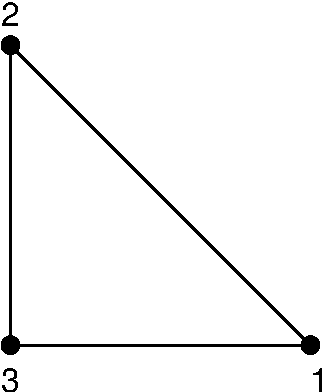
\includegraphics[width = 0.4\linewidth]{tria3.pdf}
\caption{Linear interpolation.}
\end{minipage}
\hspace{0.5cm}
\begin{minipage}[b]{0.5\linewidth}
\centering
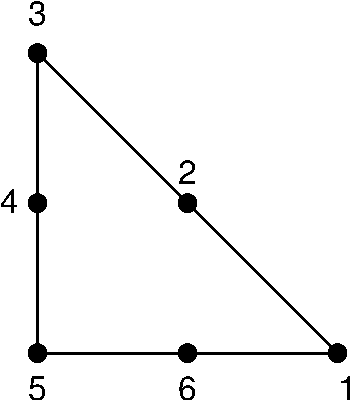
\includegraphics[width = 0.4\linewidth]{tria6.pdf}
\caption{Quadratic interpolation.}
\end{minipage}
\end{figure}

Using this convention the shape functions for the linear case are simply given by:

\begin{eqnarray}
N_1 & = & L_1 \\
N_2 & = & L_2 \\
N_3 & = & 1-L_1-L_2
\end{eqnarray}

Under this convention the quadratic interpolation shape functions are given by:

\begin{eqnarray}
N_1 & = & L_1(2L_1-1) \\
N_2 & = & 4L_1L_2 \\
N_3 & = & L_2(2L_2-1) \\
N_4 & = & 4L2(1-L_1-L_2) \\
N_5 & = & L_3[1-2(L_1+L_2)] \\
N_6 & = & 4L_1(1-L_1-L_2)
\end{eqnarray}

\pagebreak
\section{Numerical Integration}

\subsection*{Regular integrals}
For non-singular integrals the integration is done using gaussian quadrature with NG integration points per element as in:

\begin{equation}
\int_{-1}^1{F(L_1,L_2)dL_1dL_2} \approx \sum_{i=1}^{NG}{F(L_1^i,L_2^i)w_i}
\end{equation}

By default the program uses 7 points per triangular element. Tests where done with 16 and 64 points per element and the accuracy of the results was not affected, so 7 points were kept for speed.

\subsection*{Weakly singular integrals}
For weakly singular integrals the integration is done through a regularization transformation that eliminates the singularity. The element is transformed into a triangle with a singularity in node 1 and then into a degenerate square. In the degenerate square we can use Gauss-Jacobi integration to integrate getting rid of the singularity. See Figure 3 for the transformation.

\begin{equation}
\int_{-1}^1{F(L_1,L_2)(1+L_2)dL_1dL_2} \approx \sum_{i=1}^{NG}{\sum_{j=1}^{NG}{F(L_1^i,L_2^j)w_i^{\rm Gauss}w_j^{\rm Gauss-Jacobi}}}
\end{equation}

Notice that the Gauss-Jacobi integration is necessary in only one of the directions, so in the other the standard Gauss quadrature on a line is used and the product of the two provides the correct integration as indicated by the expression above.

\begin{figure}[!hbt]
\begin{center}
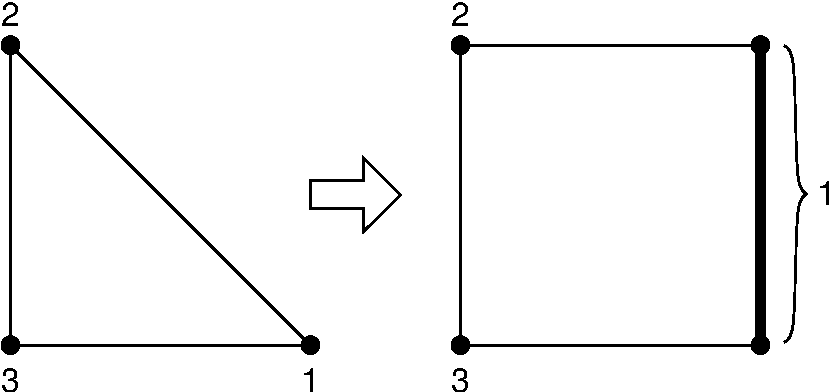
\includegraphics[width=0.6\textwidth, viewport = 0 0 402 188]{weakly_singular.pdf}
\caption{Regularization transformation for weakly singular integrals (linear case).}
\end{center}
\end{figure}

In the case of quadratic triangles when the singular point is on an edge of the triangle rather than on a vertex the triangle is divided in two and then the same regularization procedure is applied to both subtriangles as shown in Figure 4.

\begin{figure}[!hbt]
\begin{center}
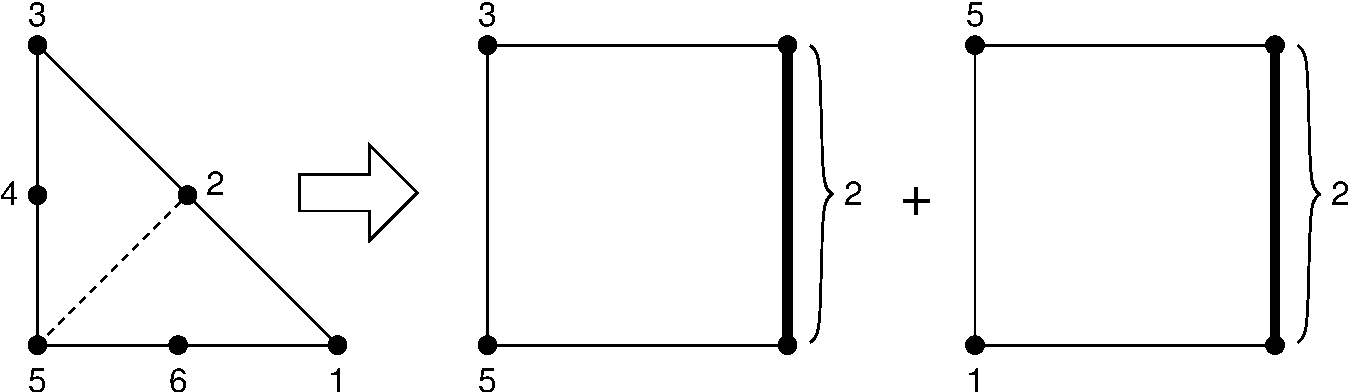
\includegraphics[width=\textwidth]{weakly_singular_t6.pdf}
\caption{Regularization transformation for weakly singular integrals (quadratic case).}
\end{center}
\end{figure}

\subsection*{Strongly singular integrals}
For strongly singular integrals we subdivide the triangle progressively in up to \verb+NSUBDIVISIONS+ --found in file \verb+constants.h+-- subsequent divisions, and integrate using standard gausian quadrature in each subtriangle except the closest to the singular point, which is neglected (it can be shown that the integrand goes to zero very close to the singularity point). The subdivision process is ilustrated in Figure 5 for a singularity at node 3 in a flat triangle.

\begin{figure}[!hbt]
\begin{center}
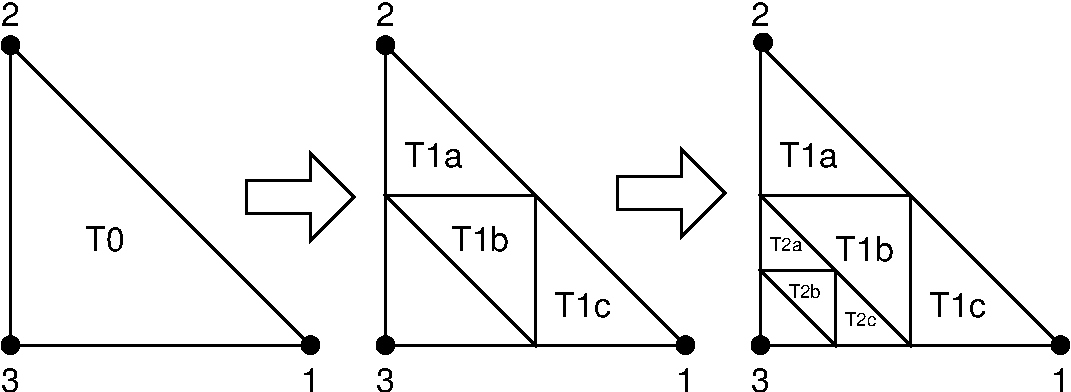
\includegraphics[width=\textwidth]{strongly_singular.pdf}
\caption{Subdivision process for strongly singular integrands with singularity at node 3 (only two consecutive subdivisions shown).}
\end{center}
\end{figure}

In the cases where the singular point is on the edge of a quadratic element rather than on a vertex the triangle is divided in two and the same subdivision process applied to the resulting subtriangles.

\subsection*{Changing the number of integration points}
The gaussian quadrature data is stored in the file \verb+gaussData.h+, and has two options, one with 7 integration points and another one with 64 integrations points. By default the code uses 7 integration points because increasing this number does not seem to improve accuracy, but this can be changed by following these stpdf:

\begin{enumerate}
\item Change the value of \verb+TNGAUSS+ and \verb+TSNGAUSS+ to 64 in file \verb+constants.h+
\item Comment out the 7 point \verb+TGauss+ and \verb+TSGauss+ matrices in file \verb+gaussData.h+
\item Uncomment the 64 point \verb+TGauss+ and \verb+TSGauss+ matrices in file \verb+gaussData.h+
\item Recompile the source code
\end{enumerate}

The constant values \verb+TNGAUSS+ and \verb+TSNGAUSS+ are the number of integration points in regular and strongly singular integrals, so it is also possible to use different values for them. Keep in mind that \verb+NSUBDIVISIONS+ are made in the case of strongly singular integrals, and therefore many more points are used for the integration even if \verb+TNGAUSS+ and \verb+TSNGAUSS+ are given the same value.

The numerical values of the gaussian integration are shown in the following tables.

\pagebreak
\begin{center}
\begin{tabular}{|c|c|c|c|}
\multicolumn{4}{c}{Table 1: Abscissas and weights for Gauss quadrature on a triangle}\\
\hline
NG & $x_i$ & $y_i$ & $w_i$\\
\hline\hline
7 & 0.333333333333333 & 0.333333333333333 & 0.112500000000000\\
 & 0.470142064105115 & 0.470142064105115 & 0.066197076394253\\
 & 0.059715871789770 & 0.470142064105115 & 0.066197076394253\\
 & 0.470142064105115 & 0.059715871789770 & 0.066197076394253\\
 & 0.101286507323456 & 0.101286507323456 & 0.062969590272414\\
 & 0.797426985353088 & 0.101286507323456 & 0.062969590272414\\
 & 0.101286507323456 & 0.797426985353088 & 0.062969590272414\\
  \hline
\end{tabular}
\end{center}

\begin{center}
\begin{tabular}{|c|c|c|}
\multicolumn{3}{c}{Table 2: Abscissas and weights for Gauss-Jacobi quadrature on a line}\\
\hline
NG & $x_i$ & $w_i$\\
\hline\hline
8 & -0.910732089420060 & 0.013180765768995\\
 & -0.711267485915709 & 0.713716106239446\\
 & -0.426350485711139 & 0.181757278018796\\
 & -0.090373369606853 & 0.316798397969277\\
 & 0.256135670833455 & 0.424189437743720\\
 & 0.571383041208738 & 0.450023197883551\\
 & 0.817352784200412 & 0.364476094545495\\
 & 0.964440169705273 & 0.178203217446225\\
\hline
\end{tabular}
\end{center}

\begin{center}
\begin{tabular}{|c|c|c|}
\multicolumn{3}{c}{Table 3: Abscissas and weights for Gauss quadrature on a line}\\
\hline
NG & $x_i$ & $w_i$\\
\hline\hline
8 & -0.960289856497536 & 0.101228536290370\\
 & -0.796666477413627 & 0.222381034453376\\
 & -0.525532409916329 & 0.313706645877887\\
 & -0.183434642495650 & 0.362683783378362\\
 & 0.183434642495650 & 0.362683783378362\\
 & 0.525532409916329 & 0.313706645877887\\
 & 0.796666477413627 & 0.222381034453376\\
 & 0.960289856497536 & 0.101228536290370\\
\hline
\end{tabular}
\end{center}
\end{document}
